% Left: Euclid-style construction of the regular pentagon from cos 72 = (sqrt5 - 1)/4. Right: the tower of fields Q in Q(sqrt2, sqrt3). Generated by a short script.
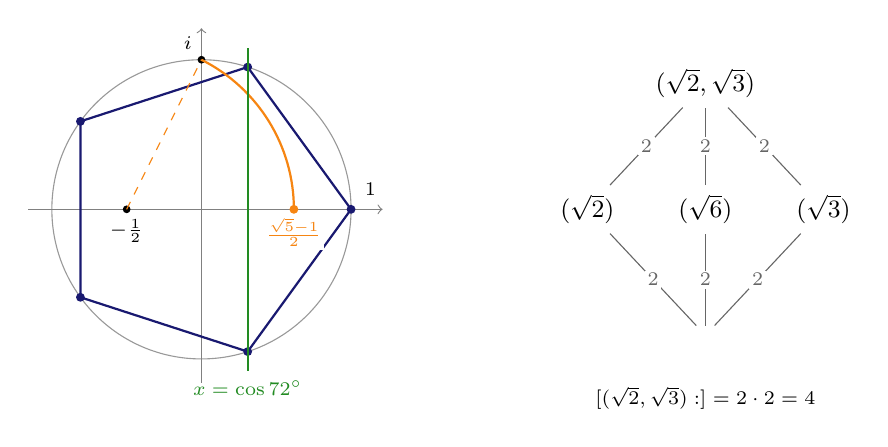
\begin{tikzpicture}
\draw[black!40] (0,0) circle (1.9);
\draw[->,black!50] (-2.20,0) -- (2.30,0);
\draw[->,black!50] (0,-2.20) -- (0,2.30);
\draw[thick,MidnightBlue] (1.900,0.000) -- (0.587,1.807) -- (-1.537,1.117) -- (-1.537,-1.117) -- (0.587,-1.807) -- cycle;
\fill[MidnightBlue] (1.900,0.000) circle (1.6pt);
\fill[MidnightBlue] (0.587,1.807) circle (1.6pt);
\fill[MidnightBlue] (-1.537,1.117) circle (1.6pt);
\fill[MidnightBlue] (-1.537,-1.117) circle (1.6pt);
\fill[MidnightBlue] (0.587,-1.807) circle (1.6pt);
\fill (0,1.900) circle (1.4pt) node[above left,font=\scriptsize] {$i$};
\fill (-0.950,0) circle (1.4pt) node[below,font=\scriptsize] {$-\frac12$};
\draw[BurntOrange,thick] (-0.950,0) ++(63.43:2.124) arc (63.43:0:2.124);
\draw[BurntOrange,dashed] (-0.950,0) -- (0,1.900);
\fill[BurntOrange] (1.174,0) circle (1.6pt) node[below=2pt,font=\scriptsize,text=BurntOrange,fill=white,inner sep=1pt] {$\frac{\sqrt5-1}2$};
\draw[ForestGreen,thick] (0.587,-2.050) -- (0.587,2.050);
\node[font=\scriptsize,text=ForestGreen,anchor=north] at (0.587,-2.050) {$x=\cos72^\circ$};
\node[font=\scriptsize,anchor=west] at (1.950,0.25) {$1$};
\node[font=\small] (Q) at (6.4,-1.6) {$\Q$};
\node[font=\small] (a) at (4.9,0) {$\Q(\sqrt2)$};
\node[font=\small] (b) at (6.4,0) {$\Q(\sqrt6)$};
\node[font=\small] (c) at (7.9,0) {$\Q(\sqrt3)$};
\node[font=\small] (L) at (6.4,1.6) {$\Q(\sqrt2,\sqrt3)$};
\draw[black!60] (Q) -- node[font=\scriptsize,fill=white,inner sep=1pt] {$2$} (a);
\draw[black!60] (Q) -- node[font=\scriptsize,fill=white,inner sep=1pt] {$2$} (b);
\draw[black!60] (Q) -- node[font=\scriptsize,fill=white,inner sep=1pt] {$2$} (c);
\draw[black!60] (a) -- node[font=\scriptsize,fill=white,inner sep=1pt] {$2$} (L);
\draw[black!60] (b) -- node[font=\scriptsize,fill=white,inner sep=1pt] {$2$} (L);
\draw[black!60] (c) -- node[font=\scriptsize,fill=white,inner sep=1pt] {$2$} (L);
\node[font=\scriptsize,align=center] at (6.4,-2.4) {$[\Q(\sqrt2,\sqrt3):\Q]=2\cdot2=4$};
\end{tikzpicture}
